\documentclass[a4paper, 11pt]{article}
 
\usepackage[utf8]{inputenc}
\usepackage{graphicx}
\usepackage[frenchb]{babel}
\usepackage{tikz}
\usetikzlibrary{arrows,automata}
\usepackage{makecell}

\begin{document}
 
\title{SPECIF\\Compte-rendu de TME}
\author{Redha Gouicem}
\date{03/03/2015}
 
\maketitle
 
\section{Métronome}
\paragraph{Question 1}
L'automate généré par la commande \texttt{lus2oc -0} contient un unique noeud muni d'une unique transition vers 
lui-même. 

\paragraph{Question 2}
On fait d'abord la correspondance entre les variables du code \texttt{C} et les variables du code 
\texttt{lustre}.
\begin{itemize}
  \item V1 : reset
  \item V2 : delay
  \item V3 : true$\rightarrow$false
  \item V4 : first
  \item V5 : n
  \item V6 : hz
  \item V7 : state
  \item V8 : tic
  \item V9 : tac
\end{itemize}

\paragraph{}
Soit $D = \{premier\_cycle, first, hz, n, state, tic, tac\}$, avec $premier\_cycle$ initialisé à \texttt{true}.

\begin{tikzpicture}[->,>=stealth',shorten >=1pt,auto,node distance=2.8cm,
                    semithick]
  \tikzstyle{every state}=[fill=white,text=black]

  \node[initial,state] (s0) {$s_0$};
  \path (s0) edge [loop right] node 
        {\makecell[l]{[true]\\
            first $\leftarrow$ \textbf{if} premier\_cycle \textbf{then} false \textbf{else} first $||$ reset;\\
            hz $\leftarrow$ \textbf{if} premier\_cycle \textbf{then} 0 \textbf{else} (\textbf{if} reset \textbf{then} delay \textbf{else} hz);\\
            n $\leftarrow$ \textbf{if} premier\_cycle \textbf{then} 0 \textbf{else} (\textbf{if} n $<$ 0 \textbf{then} n-1 \textbf{else} hz-1;\\
            state $\leftarrow$ \textbf{if} premier\_cycle \textbf{then} false \textbf{else} (\textbf{if} n $<$ 1 \textbf{then} !state \textbf{else} state;\\
            tic $\leftarrow$ \textbf{if} premier\_cycle \textbf{then} false \textbf{else} first \&\& n $<$ 1 \&\& state \&\& hz $>$ 0;\\
            tac $\leftarrow$ \textbf{if} premier\_cycle \textbf{then} false \textbf{else} first \&\& n $<$ 1 \&\& !state \&\& hz $>$ 0;\\
            premier\_cycle $\leftarrow$ false;}} (s0);
\end{tikzpicture}

\paragraph{Question 3}
L'automate généré avec \texttt{lus2oc -2} contient 5 noeuds. On peut identifier les variables suivantes :
 \begin{itemize}
  \item V1 : reset
  \item V2 : delay
  \item V3 : hz $>$ 0
  \item V4 : hz
  \item V5 : n $<$ 1
  \item V6 : n
  \item V7 : n $>$ 0
  \item V8 : tic
  \item V9 : tac
\end{itemize}
\paragraph{}
On en déduit que l'automate a été déplié selon les variables \texttt{first}, \texttt{state} et \texttt{premier\_cycle}.

\section{Feux de voiture (version étendue)}
\paragraph{Comportement testé avec \texttt{luciole}}
\begin{center}
  \makebox[\textwidth]{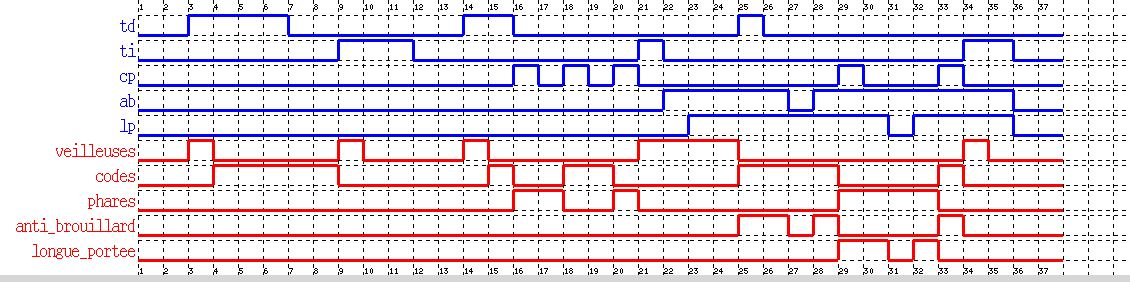
\includegraphics[width=\paperwidth]{feux_etendue.png}}
\end{center}

\end{document}
